\chapter{Background}
\label{Chapter4}

In this section we're going to review the concepts required to understand the SVM-RFE algorithm. Section \ref{sec:context} already introduced some concepts around the SVM-RFE algorithm, placed it in context, and enumerated some of its applications. In this section we'll focus on the inner workings of the algorithm and how these parts add together. 

\section{Machine learning}

Machine learning is a subfield in the broader discipline that is artificial intelligence, with a particular take in statistics. These algorithms, also called learning machines or just machines, use data to learn patterns and make predictions. The data is collected in a separated unrelated process, and structured in the form of a \emph{dataset} (a collection of data). Once the dataset is further cleaned and prepared, the learning machine finally consumes it in a process called \emph{training}. After this process the machine pro\-duces a \emph{model}, which is a function that can be used to make predictions on new data.

Two canonical problems in machine learning are regression and classification problems.

\subsection{The dataset}

A dataset is simply a collection of data. In the context of machine learning this data-set will be used to make predictions, take decisions, or find patterns. For a machine learning algorithm to be able to consume a dataset the first step is to represent it in tabular form. 

Most datasets come already in tabular form. Some of the most notable ex\-cep\-tions are datasets involving images. In this case computer vision methods are often used to extract numeric data representing characteristics of the image. Sometimes a more direct transformation can also be made, for example making each feature be the intensity level of a single pixel in the image. This of course produces a high number of features, most of which are redundant or irrelevant (e.g. features representing pixels in the background). 

In a dataset represented as a table, columns describe different \emph{features}, \emph{properties} or \emph{attributes} of some group of objects and rows represent \emph{instances} or \emph{examples} of that group. For example, if objects were vehicles then features could include the brand, power, weight, max\-imum speed, and other such characteristics of various vehicles, each of which would be in a row. Different names are used in different contexts. One of the most typical naming conventions comes from the statistics domain which refers to columns as \emph{variables} and rows as \emph{observations}. Sometimes different nomenclature is used to differentiate features in different stages of the cleaning and preparation process, but in this thesis we use them all instinctively.

\begin{table}[h]
    \makebox[\textwidth][c]{
        \begin{tabular}{l l l l l l l l l}
        \toprule
        \tabhead{Src} & \tabhead{Dst} & \tabhead{NAT-Src} & \tabhead{NAT-Dst} & \tabhead{Action} & \tabhead{Sent (B)} & \tabhead{Rcvd. (B)} & \tabhead{Packets} & \tabhead{Elapsed (sec)}\\
        \midrule
        57222 & 53 & 54587 & 53 & allow & 94 & 83 & 2 & 30 \\
        56258 & 3389 & 56258 & 3389 & allow & 1600 & 3168 & 19 & 17 \\
        6881 & 50321 & 43265 & 50321 & allow & 118 & 120 & 2 & 1199 \\
        43537 & 2323 & 0 & 0 & deny & 60 & 0 & 1 & 0 \\
        50002 & 443 & 45848 & 443 & allow & 6778 & 18580 & 31 & 16 \\
        \bottomrule\\
        \end{tabular}
    }
    \caption{Example dataset extracted from the Internet Firewall Data (\cite{ertam_internet_2019}). Only five observations and main variables shown. }
    \label{tab:example_dataset}
\end{table}

\subsection{Classification}
\label{sec:ch4.classification}

For the classification problem we want to predict in witch group or \emph{class} to assign some new observation. Table \ref{tab:example_dataset} provides an example of what could be a good classification problem. Imagine we are building a firewall and want it to predict if some new packet in the network should be allowed to pass. We could train a classification learning machine with the dataset represented in the table (the full version) and produce a model capable of doing such predictions. Although it is trivial to identify a pattern in the example, it may not be so for real world examples. Automatic \emph{pattern recognition} is key in solving many real world problems, and it is one of the features of these algorithms.

Mathematically, the set of observations is defined as $X = \{\vt{x_1}, \vt{x_2}, \dots, \vt{x_n}\}$ and the set of the corresponding labels or target classes is $y = \{y_1, y_2, \dots, y_n\}$ with every element of this set being some class $y_i = C_k$ of a discrete set of classes with size $K$. They are called \emph{domain set} and \emph{label set} respectively. For our example, the classes would be $C = \{\text{allow}, \text{deny}\}$. Thus, we can describe the goal of a classification problem as assigning some class $C_k$ to an input vector $\vt{x}$.

Although we've used strings to represent classes, part of the preparation process of the dataset involves turning all values into numerical scalars, so our classes would actually be some natural numbers. Also notice that every $\vt{x_i}$ is a vector containing a single numerical value for each feature excluding the label. 

We make a distinction between two-class problems (or binary) and multi-class problems. Two-class problems typically use $C = \{0, 1\}$ as classes and thus can be modeled with a boolean function or, if a probability is desired, a function that returns values between 0 and 1. This simplifies the model substantially, in fact some learning machines such as the SVM can only work with two-class problems, and use different methods to extend to the multi-class version.

\subsection{Visualization}
\label{sec:ch4.visualization}

A visualization of the problem in some euclidean space is required to understand how most classification algorithms work, and in particular SVM. Typically, clas\-si\-fi\-cation models divide the input vector space\footnote{The euclidean space of minimum dimension containing all possible input vectors $\vt{x}$.} into \emph{decision regions}. The boundaries of such regions are called \emph{decision boundaries} or \emph{decision surfaces}. If the decision boundary is in the form of some hyperplane of dimension $(D - 1)$, with $D$ being the dimension of the space, then we say that it's a linear model. A dataset whose classes can be completely separated by such linear decision boundary is said to be \emph{linearly separable}.

\begin{figure}[H]
    \centering
    \begin{subfigure}[b]{0.4\linewidth}
        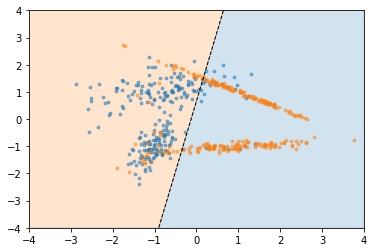
\includegraphics[width=\linewidth]{img/ch4/nolinsep.png}
        \subcaption*{Not linearly separable}
    \end{subfigure}
    \begin{subfigure}[b]{0.4\linewidth}
        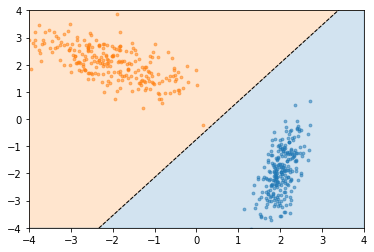
\includegraphics[width=\linewidth]{img/ch4/linsep.png}
        \subcaption*{Linearly separable}
    \end{subfigure}
    \caption{Decision regions and 1-D hyperplane boundary of some linear model for two datasets. Points are observations, colors indicate the class.}
    \label{fig:ch4.sep}
\end{figure}

Given a boundary we can determine in which region some new point $\vt{x}$ falls using a \emph{discriminant function}. One of the most trivial cases is when the boundary is lineal. It is convenient now to do a small refresh on the equation that describes a hyperplane.

\subsubsection*{Equation of a line (slope-intercept form)}
\begin{align}
    y = mx + t
\end{align}

Where $m$ is the \emph{slope} or \emph{gradient}, $x$ is the independent variable of the function $y = f(x)$ and $t$ is the y-intercept value, the point of the function where the line crosses the y-axis, i.e. $t = f(0)$. This description has the advantage that can be directly represented as a function $f(x) = mx + t$.

\subsubsection*{Equation of a line (standard form)}
\begin{align}
    ax + by = c
\end{align}

This is an equivalent form, this one however is not representable by a function $f: \mathbb{R} \rightarrow \mathbb{R}$, instead it is often represented as a set $L = \{(x, y) \st ax + by = c\}$. This allows representing vertical lines and also features the useful property that $(a, b)$ is the normal vector\footnote{A vector that is perpendicular to the surface.} of the line.

\subsubsection*{Equation of a line (general form)}
\begin{align}
    ax + by - c = 0
\end{align}

A simple linear transformation of the standard form produces the general form (\cite{noauthor_wikipedia_2021}). This conserves the normal vector and also has the advantage of being representable by an implicit function\footnote{A function of multiple variables $f: \mathbb{R}^n \rightarrow \mathbb{R}$ such that we only consider solutions where $f(X) = 0$. For example a circle can be defined with an implicit function $f(x, y) = x^2 + y^2 - r$, but if we were to plot it in 3-D we would instead see an inverted cone.}. Notice that if represented in 3-D it would produce a plane that is perpendicular to the $xy$ plane, since its normal would always have the form $(a, b, 0)$.

\subsubsection*{Equation of a 3-D Plane}
\begin{align}
    ax + by + cz + d = 0
\end{align}

We can extend the general form of a line with one more dimension, it only requires adding the new term $cz$ for the new dimension. We've also changed the sign of the constant term $d$ for compactness. This is a conceptual move, not an algebraic one.

\subsubsection*{Equation of a Hyperplane}
\begin{align}
    w_1x_1 + \dots + w_nx_n + w_0 = 0
\end{align}

This is a generalization of the equation of a 3-D plane for $n$ dimensions. It also happens to be the definition of a \emph{linear equation}. The variables $w_1, \dots, w_n$ are called \emph{coefficients}, \emph{parameters} or \emph{weights}, and the variable $w_0$ is the constant term. It is important to avoid confusing $x_i$ with $\vt{x_i}$, the first is the one the coordinates of a point in some dimension, and the other is an observation of a dataset (a point). In particular, it may be the case that $\vt{x_j} = (x_1, x_2, \dots, x_n)$.

We may want to compact this expression more by using vectors. So, another form for representing the equation of a hyperplane is:
\begin{align}
    \vb{w}^{\T}\vb{x} + w_0 = 0
\end{align}

Where $\vb{w}$ is called the \emph{vector weight} and $w_0$ the \emph{bias}. We can turn this equation into a discriminant function for two classes by simply considering what happens with points that are not in the hyperplane. By definition such points meet one of the two inequations:

\begin{align*}
    \vb{w}^{\T}\vb{x} + w_0 > 0 \\
    \vb{w}^{\T}\vb{x} + w_0 < 0
\end{align*}

A point will be a solution of one of these inequations depending on whether it is in the subspace, i.e. discriminant region, facing the direction of the normal or the opposite.

A linear binary classification learning machine is thus an algorithm that given some dataset finds appropriate values for the parameters $\vb{w}$ and $w_0$ of the hyper\-plane in order to produce a discriminant function $y : \mathbb{R}^n \rightarrow \mathbb{R}$ such as:
\begin{align}
    y(\vb{x}) = \vb{w}^{\T}\vb{x} + w_0
\end{align}

\subsection{Performance}

Usually models produced by a learning machine do not always make correct pre\-dict\-ions, instead we consider them good enough if they can classify new data correctly most of the time. In order to quantize how good of a predictor some model is we can use various performance metrics.

The most typical metric for classification problems is \emph{accuracy}. This is the ratio of correct predictions versus the total number of predictions made. The inverse to the accuracy is defined as the \emph{error}. Notice that the classification accuracy will always be some percentage above 50\%. This is because a classifier performing consistently worse than that can be turned into a good classifier by simply flipping the output of the discriminant function. Thus, the worst possible classifier is that of a coin toss, i.e. a uniform random distribution, with an expected accuracy of exactly 50\%.

In some problems a distinction is made between misclassifications depending on which class is misclassified. An example of this is how misclassifying a patient with cancer with a healthy diagnosis is worse than misclassifying a healthy patient with a cancer diagnosis, the consequence of one is potentially death due to lack of treatment while the other is simply more investigation. For these problems a quadratic amount of cases appears. For the binary classification the standard nomenclature is to name the classes \emph{positive} and \emph{negative} and then prefix them with \emph{true} or \emph{false} depending on whether the prediction was correct or not. In this way a matrix called \emph{confusion matrix} is created, with the diagonal containing all the correct predictions.

\begin{figure}[H]
    \centering
    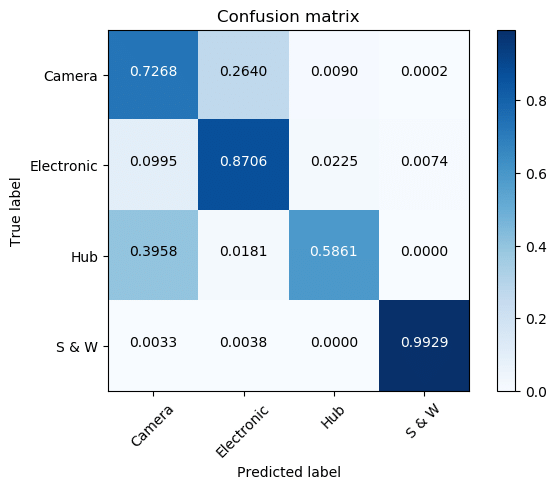
\includegraphics[width=0.5\linewidth]{img/ch4/confusion.png}
    \caption{Confusion matrix extracted from the paper “Automatic Device Classification from Network Traffic Streams of Internet of Things” (\cite{bai_automatic_2018}).}
    \label{fig:ch4.confusion}
\end{figure}

From a confusion matrix various other metrics can be extracted, such as \emph{precision}, \emph{specificity} or \emph{recall}, but it is unlikely that we make use of them in this project. Often models internally use a \emph{loss} or \emph{cost} function that they try to minimize in order to optimize the parameters, the inverse of which is called \emph{utility function}. Even if the model doesn't internally use one such function, one can be constructed form performance metrics, which is then referred as the \emph{score}. 

It is known that learning requires both \emph{generalization} and \emph{memorization}. If a model memorizes the dataset, thus has high accuracy on data already in the dataset, but doesn't generalize well, thus has low accuracy when predictions are done on new data, we say there is \emph{overfitting}. Notice that for this to be detected we must test the dataset with new data. In order to do so a dataset is often split in \emph{train} and \emph{test} subsets, and although accuracies form both subsets may be reported, only the accuracy of the test subset may be taken as good.

One of the possible causes of overfitting is the \emph{Bias-Variance} trade-off. It's an effect in which if you select a very simple model then the algorithm fails to generalize (bias) but selecting a very complex algorithm increases memorization and leads to high variability in the presence of an unseen observation (variance). The best model is thus one with a middle-ground complexity.

Selecting the complexity of an algorithm can be done with the use of some extra parameters, not fitted by the training phase of the leaning machine, that we call \emph{hyper-parameters}. The existence of this extra parameters depends on the models, some may not have any. Because these parameters modify the model, searching for the best hyper-parameters is called \emph{model selection}. Model selection is often done in a brute force manner, by simply trying different values of the hyper-parameters and selecting the ones that give the best result. Al\-though this coarse strategy is usually enough, more complex search strategies such as successive halving or genetic algo\-rithms (\cite{claesen_hyperparameter_2015}) can also be used. In the case of one single hyper-parameter we can draw a plot and visualize how the score evolves. Because model selection may be understood as some kind high level training, specially when com\-plex search strategies are used, a third division on the dataset may be made, named the \emph{validation} set.

\begin{figure}[H]
    \centering
    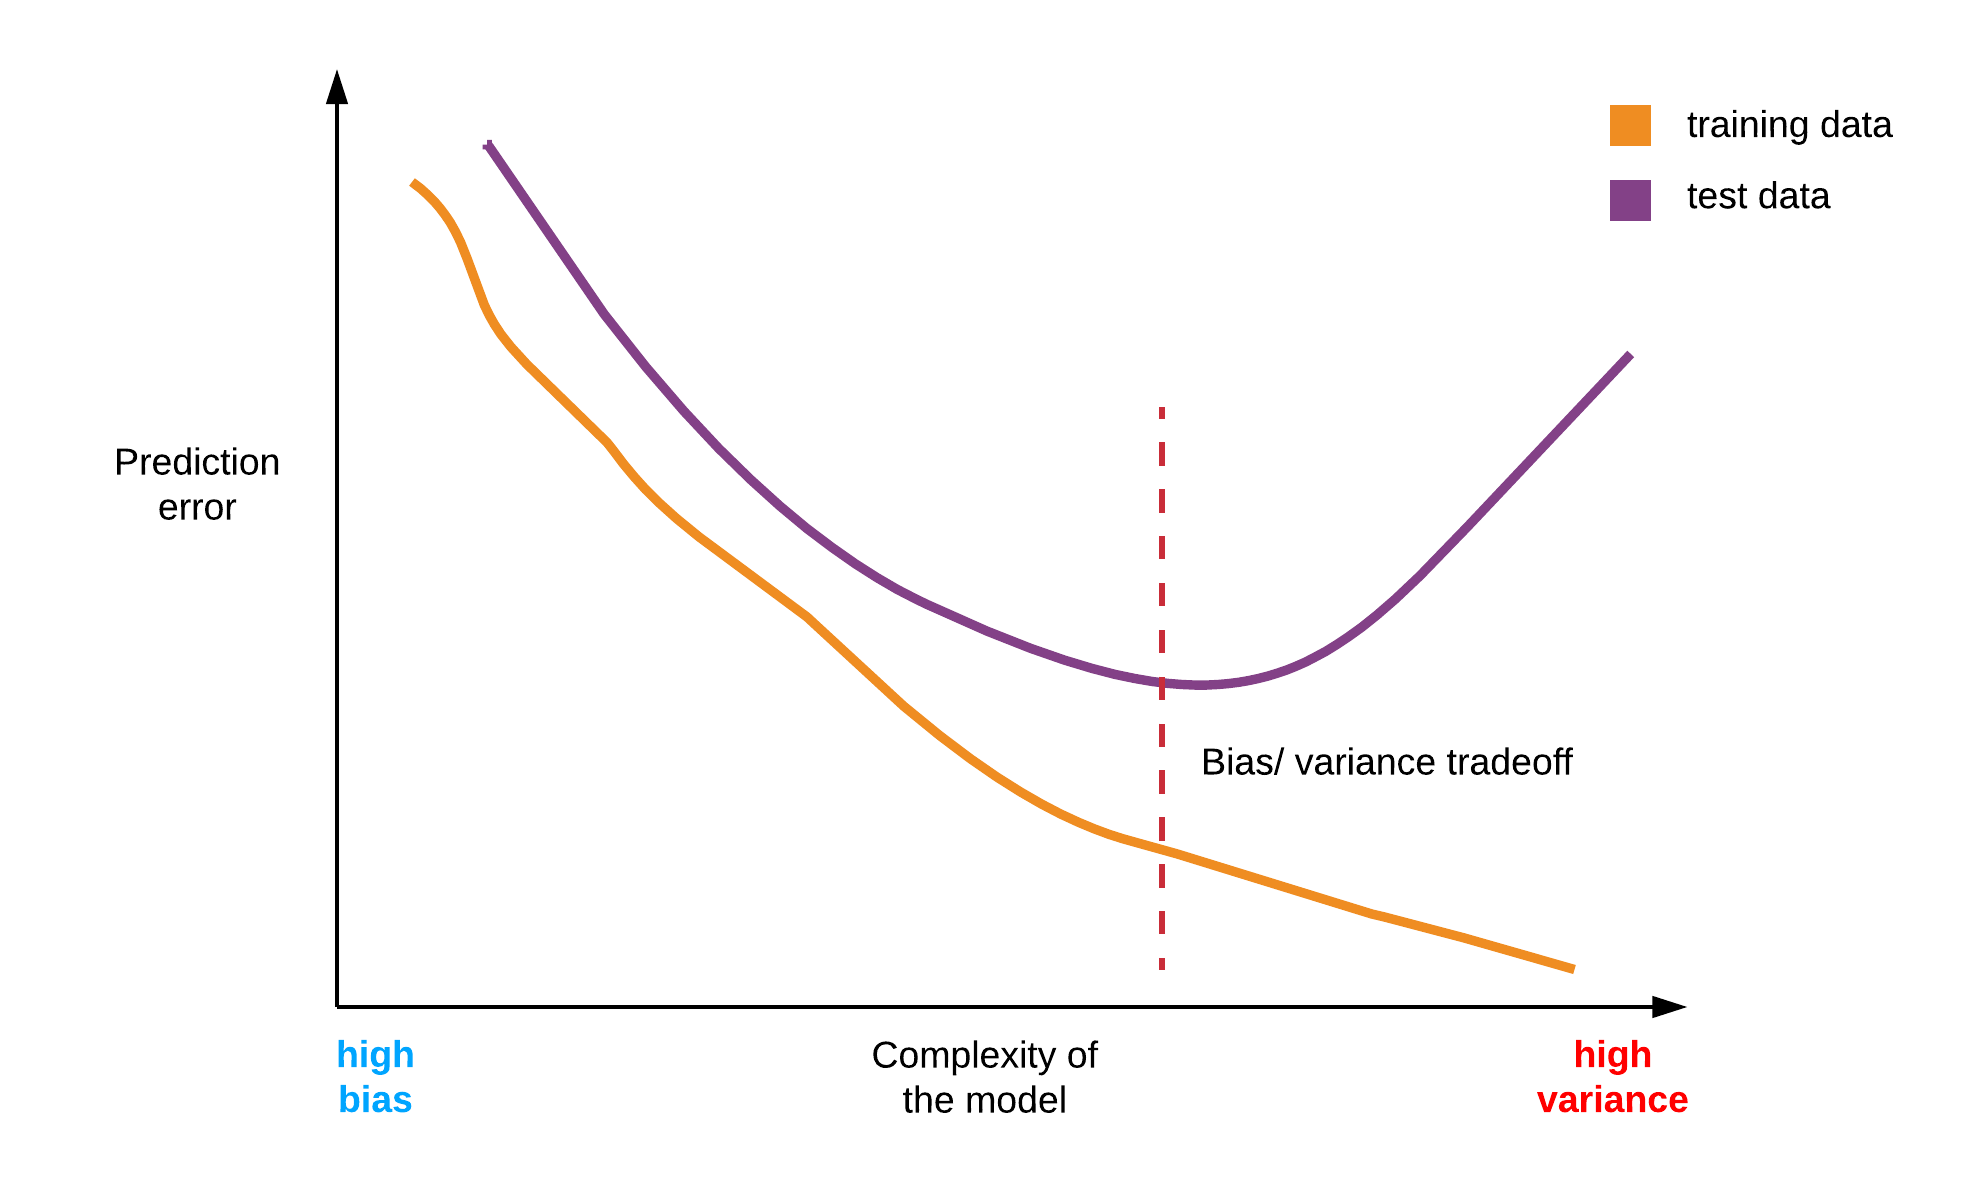
\includegraphics[width=0.5\linewidth]{img/ch4/bias-and-variance.png}
    \caption{Bias-Variance trade-off. Source (\cite{bisong_machine_2021}).}
    \label{fig:ch4.biasvariance}
\end{figure}

Machine learning algorithms work better the more observations they are trained with, however it is not often the case that we have an unlimited amount of them. In analyzing the performance of a leaning machine, or doing model selection, it may be useful to repeat the experiments multiple times with different data of the same distribution, i.e. from the same dataset. This provides second order statistics, such as the mean or the covariance, on the resulting scores, which may prove very useful to get a better idea of what is going on. This however implies further slicing the dataset in as many slices as experiments one wants to do. After so much slicing, the remaining training subsets would often contain very few observations, thus reducing the performance of the models and nullifying the advantages of having a probability distribution on the scores. 

A method called \emph{cross-validation} can be used to make mul\-ti\-ple experiments with\-out increasing the amount of data. The method first makes $K$ partitions called \emph{folds}. For each fold, one experiment is made such that the fold is used as the validation set and the remaining folds become the training set. This allows a portion $(K-1)/K$ of the observations to be used for training in each run and allows assessing performance using the whole dataset. In the particular case where $K = N$, useful for when the amount of observations is really low, we name this method \emph{leave-one-out} cross-validation. It is also possible to shuffle the data, which allows even more re-utilization. Although this method is computationally expensive (since it requires running the whole experiment $K$ times), it has the advantage of being trivial to parallelize, and thus it can run at increased speeds in computers with a multi-core CPU architecture. 

\section{Support Vector Machines}

As it has been discussed in section \ref{sec:ch4.visualization}, the decision boundary of a binary class\-ification prob\-lem may be represented with a hyperplane, and it is the weights of this hyperplane what the learning machine tries to fit such that the hyper\-plane correctly separates the two classes. There may be infinitely many hyperplanes that correctly separate the examples of two classes, but some of them are better suited than others. For the purpose of generalization, we want decision regions that can accommodate new data outside the convex hulls\footnote{In geometry, the \emph{convex hull} or \emph{convex envelope} of a shape is the smallest convex set that contains it.} of each group of examples. That is, we want some kind of separation between the hyperplane and the observations.

\begin{figure}[H]
    \centering
    \begin{subfigure}[b]{0.4\linewidth}
        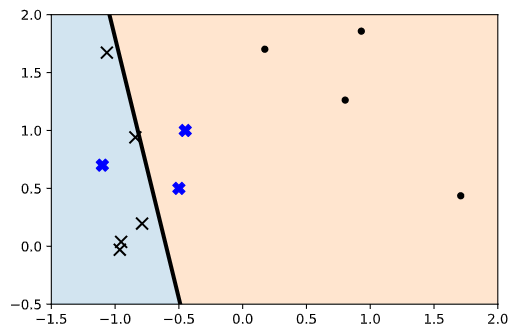
\includegraphics[width=\linewidth]{img/ch4/boundrybad.png}
        \subcaption*{Bad boundary}
    \end{subfigure}
    \begin{subfigure}[b]{0.4\linewidth}
        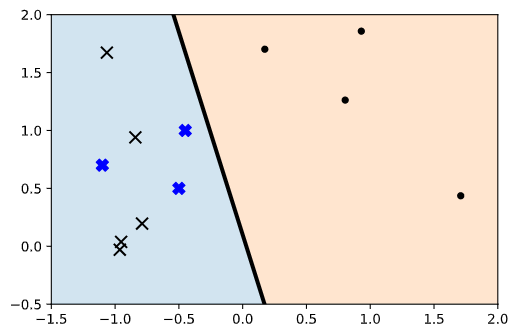
\includegraphics[width=\linewidth]{img/ch4/boundrygood.png}
        \subcaption*{Good boundary}
    \end{subfigure}
    \caption{Showing how one decision boundary may be better than another. \texttt{X} filled in blue represents new data.}
    \label{fig:ch4.sep}
\end{figure}

There exist various learning machines that accomplish this separation, e.g. the \emph{Fisher’s linear discriminant}. Another such machine is the Support Vector Machine (SVM), which is based on the idea of finding the biggest margin between the extreme points of each class and setting the decision boundary in the center of such margin. For this reason SVM machines are said to be \emph{Maximum Margin Classifiers}.

\begin{figure}[H]
    \centering
    \begin{subfigure}[b]{0.4\linewidth}
        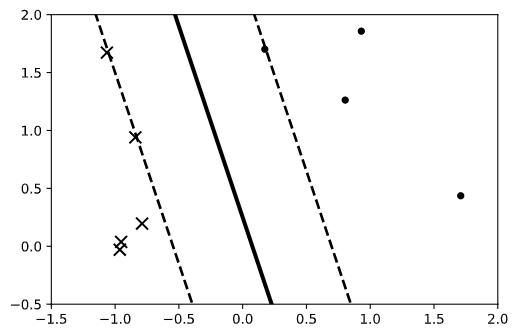
\includegraphics[width=\linewidth]{img/ch4/mmc_good.png}
        \subcaption*{Maximum margin}
    \end{subfigure}
    \begin{subfigure}[b]{0.4\linewidth}
        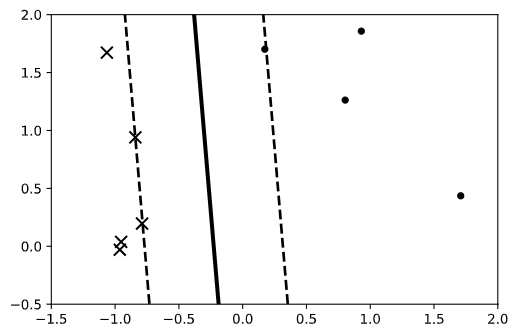
\includegraphics[width=\linewidth]{img/ch4/mmc_bad.png}
        \subcaption*{Quite good margin}
    \end{subfigure}
    \caption{Two quite good decision boundaries with a margin, a maximum margin classifier would choose the left one.}
    \label{fig:ch4.sep}
\end{figure}

The \emph{margin} is defined as the perpendicular distance (i.e. in the direction of the normal) between the decision bound\-ary and the closest of the examples. There is only one decision boundary that maximizes the margin. Only a limited amount of examples, defined by the number of dimensions, will reach the limits of that margin (and thus be the closest), these are called the \emph{support vectors}.

\subsection{Discriminant function}

We've already seen how to we can build a discriminant function from the equation of the hyperplane. Here we will explore this in a bit more depth and take a different approx. 

Given a vector of unknown length $\vt{w}$ that is perpendicular to the hyperplane (thus the normal) such that its origin is at the origin of the coordinate system. And given another vector $\vt{x}$ also with origin at the origin of the coordinate system. Notice that, by how we are defining them, they are actually points, but we may want to think of them as vectors for now. We are interested in knowing in which decision region the point $\vt{x}$ is placed.

To do so, we make the dot product between $\vt{w}$ and $\vt{x}$, which, in particular, will give us a scalar corresponding to the length of the projection of $\vt{x}$ over $\vt{w}$. Notice that for points within the hyperplane that length will be some constant value $c$. Thus, we can know if point $\vt{x}$ is in one region or another by comparing it with $c$. This can be expressed with the inequality $\vt{w} \cdot \vt{x} \ge c$. By making a variable $b = -c$ and expressing the dot product as a product of matrices, we can conveniently rearrange this equation as the decision rule:
\begin{align}\label{eq:drule}
    \vb{w}^\T \vb{x} + b \ge 0
\end{align}
This is analogous to the decision rule found in section \ref{sec:ch4.visualization}, in fact if we make an equality instead of an inequality we discover the equation of the hyperplane, from there we could do the process in reverse until we find the general equation of a line. 

\subsection{Margin formalization}

Notice from equation \ref{eq:drule} that the constant value of $b$ depends directly on the length $||\vt{w}||$, and because this length is not limited (there are infinite vectors that are normal to the hyperplane), an infinite amount of combinations exists.

Therefore, we may want to restrict the decision rule to a single combination. Also, it is convenient that this restriction takes such a form that allows defining the margin. First we assign to our classes the numerical values $C = \{-1, 1\}$. Then we impose the condition that points in a decision region outside the margin must have values greater than $\pm 1$, thus for points $\vb{x}_{(+)}$ in class “$1$” and $\vb{x}_{(-)}$ in class “$-1$” we get:
\begin{align*}
    \vb{w}^\T \vb{x}_{(+)} + b &\ge 1\\
    \vb{w}^\T \vb{x}_{(-)} + b &\le -1
\end{align*}

This pair of equations can be simplified to a single equation by considering the vector $\vt{y}$ that we defined in section \ref{sec:ch4.classification}. Because of the numerical values we've assigned to the classes, it will contain elements such that every $y_i \in \{-1, 1\}$. Notice that if we multiply both sides by $y_i$ (and given that we know what the value of $y_i$ will be in each case), we can produce the single equation:
\begin{align}\label{eq:svmconstrain}
    y_i (\vb{w}^\T \vb{x_i} + b) \ge 1
\end{align}

From this equation we may find the values of the hyperplanes that border the margin (named \emph{gutter}), that is, the points where the last equation is exactly 1. 

\subsubsection*{Equation of the gutters}
\begin{align}\label{eq:gutters}
    y_i (\vb{w}^\T \vb{x_i} + b) -1 = 0
\end{align}

Although now we know the equation for the gutters (analogy for the margin being a street), what we're really interested about is in the distance between them. We can calculate that distance as the diff\-erence vector form any two points in the gutters projected using the unit vector of $\vt{w}$:
\begin{align*}
    (\vt{x}_{(+)} - \vt{x}_{(-)}) \cdot \frac{\vt{w}}{||\vt{w}||}
\end{align*}

Notice that form equation \ref{eq:gutters} we can derive $\vt{w} \cdot \vt{x}_{(+)} = 1 - b$ and $\vt{w} \cdot \vt{x}_{(-)} = b - 1$, applying the distributive property we obtain:
\begin{align*}
    \frac{(1 - b) - (b - 1)}{||\vt{w}||} \implies \frac{2}{||\vt{w}||}
\end{align*}

Since we've defined the margin to be the distance from the decision boundary to a gutter (i.e. where support vectors are), and since the decision boundary is at the same distance to both gutters, then we can see that the length of the margin will be half the distance between the gutters.

\subsubsection*{Length of the margin}

\begin{align}
    \frac{1}{||\vt{w}||} = \frac{1}{\sqrt{\vb{w}^\T \vb{w}}}
\end{align}

\subsection{Optimization problem}

The problem of finding the greatest margin can be formulated as an optimization problem. Specifically we want to maximize $1/||\vt{w}||$ subject to the constraints defined in equation \ref{eq:svmconstrain}. This is equivalent to minimizing $||\vt{w}||$ subject to the same constraints. For mathematical convenience (which we will see later), we can also divide by 2 and square the objective function without it affecting the optimal solution.

\subsubsection*{Primal form}
\begin{align}\label{eq:svm_primal} 
    \underset{\vt{w}, b}{\text{arg} \min}\ \frac{1}{2} ||\vt{w}||^2 \text{\quad s.t. \quad} \forall i : y_i (\vb{w}^\T \vb{x_i} + b) - 1 \ge 0
\end{align}

This is a constrained quadratic optimization problem. There are various known algorithms that can solve constrained optimization problems, such as the \emph{simplex} algorithm. However, in our case it may be appropriate to use the \emph{Lagrangian} method. This method doesn't directly return a solution, instead it transforms the problem into another version, from which a direct solution may be more easily computed.

\subsubsection*{Lagrangian}

Imagine we had an easier optimization problem. E.g. a maximization pro\-blem such that its optimization function $f : \R^{D-1} \rightarrow \R$ is a function $f(\vt{x})$ of $D$ dimensions, and it has a single equality constrain $g(\vt{x}) = 0$ of $D - 1$ dimensions. Notice how the constraint is “projected” on top of $f(\vt{x})$. Then the Lagrangian method consists on optimizing a new function (equation \ref{eq:lagrangian_base}), via introducing a new pa\-ram\-e\-ter $\lambda$ called the \emph{Lagrangian multiplier}. 
\begin{align}\label{eq:lagrangian_base} 
    L(\vt{x}, \lambda) = f(x) - \lambda g(x)
\end{align}

Notice how there is only a subset of the images of $f(\vt{x})$ for which $f$ and $g$ inter\-sect. Where the intersection is defined as $\{\vt{x} \in \R^{D-1}\ |\ \exists \vt{c} : f(\vt{x}) = c \land g(\vt{x}) = 0\}$. Many values of $c$ contribute to the intersection, however we are only interested in the maximum or minimum values, since for these $\vt{x}$ becomes a \emph{stationary point}.

An interesting property of these functions is that in the stationary points the di\-rec\-tion of the normal of both functions must be the same. Note that if the normal of $f$ was not orthogonal to the surface of $g$, we could increase $c$ by moving a short distance along the constraint surface. Also remember that the normal is the same as the gradient of that function, i.e. $\nabla f$. Therefore, there must exist a parameter $\lambda \neq 0$ (or $\lambda > 0$ for a minimization problem) such that:
\begin{align}
    \nabla f - \lambda \nabla g = 0
\end{align}

From this we see that the constrained stationary condition is obtained by setting $\nabla_x L = 0$. Notice that the gradient is defined as the partial derivatives of each coordinate in the vector, that is:
\begin{align*}
    \nabla_x L = \left( \frac{\partial L}{\partial x_1}, \frac{\partial L}{\partial x_2}, \cdots, \frac{\partial L}{\partial x_n} \right)
\end{align*}

At first glance it may look overwhelming, but given that $L$ is the same for all $x_i$ and that we can reuse the arithmetic operators for operations between vectors, doing the gradient is very similar than doing the partial derivate over a single scalar. 

Going back to the SVM formalization, we can define the Lagrangian of the primal form (equation \ref{eq:svm_primal}) as:
\begin{align}\label{eq:svm_lagrangian_from_primal}
    L(\vt{w}, b, \vt{\alpha}) = \frac{1}{2} ||\vt{w}||^2 - \sum \alpha_i \left[ y_i (\vb{w}^\T \vb{x_i} + b) - 1\right]
\end{align}

Now we want to take the partial derivative with respect to $\vt{x}$ and equal to 0. Note that $||\vt{w}|| = \sqrt{w_1^2, w_2^2, \dots, w_n^2}$, if we elevate this expression to the power of two we can eliminate the square root, then if we divide by 2 we get a vector $\left( \frac{1}{2} w_1^2, \dots, \frac{1}{2} w_n^2 \right)$ which by deviating each coordinate we get $\vt{w}$. Therefore:
\begin{align}\label{eq:svm_representer}
    \frac{\partial L}{\partial \vt{w}} = \vt{w} - \sum \alpha_i y_i \vt{x_i} = 0 \implies \vt{w} = \sum \alpha_i y_i \vt{x_i}
\end{align}

Also, by doing the gradient with respect to $b$ and comparing with 0 we get:
\begin{align}
    \frac{\partial L}{\partial b} = - \sum \alpha_i y_i = 0 \implies \sum \alpha_i y_i = 0
\end{align}
 
If we plug these expressions back in equation \ref{eq:svm_lagrangian_from_primal} we can construct the \emph{dual form}. Note that $     ||\vt{w}||^2 = \vb{w}^\T \vb{w}$.

\begin{align*}
    L &= \frac{1}{2} \left( \sum \alpha_i y_i \vt{x_i} \right) \cdot \left( \sum \alpha_j y_j \vt{x_j} \right)
    - \sum \alpha_i \left[ y_i (\vb{w}^\T \vb{x_i} + b) - 1\right]
\\
    L &= \frac{1}{2} \left( \sum \alpha_i y_i \vt{x_i} \right) \cdot \left( \sum \alpha_j y_j \vt{x_j} \right)
    - \sum \alpha_i \left[ y_i \vb{w}^\T \vb{x_i} + y_i b - 1\right]
\\
    L &= \frac{1}{2} \left( \sum \alpha_i y_i \vt{x_i} \right) \cdot \left( \sum \alpha_j y_j \vt{x_j} \right)
    - \sum \left[ \alpha_i y_i \vb{w}^\T \vb{x_i} + \alpha_i y_i b - \alpha_i \right]
\\
    L &= \frac{1}{2} \left( \sum \alpha_i y_i \vt{x_i} \right) \cdot \left( \sum \alpha_j y_j \vt{x_j} \right)
    - \sum \alpha_i y_i \vb{w}^\T \vb{x_i} - \sum \alpha_i y_i b + \sum \alpha_i
\\
    L &= \frac{1}{2} \left( \sum \alpha_i y_i \vt{x_i} \right) \cdot \left( \sum \alpha_j y_j \vt{x_j} \right)
    - \sum \alpha_i y_i \vb{w}^\T \vb{x_i} - b \sum \alpha_i y_i + \sum \alpha_i 
\\
    L &= \frac{1}{2} \left( \sum \alpha_i y_i \vt{x_i} \right) \cdot \left( \sum \alpha_j y_j \vt{x_j} \right)
    - \sum \alpha_i y_i \vb{w}^\T \vb{x_i} + \sum \alpha_i 
\\
    L &= \frac{1}{2} \left( \sum \alpha_i y_i \vt{x_i} \right) \cdot \left( \sum \alpha_j y_j \vt{x_j} \right)
    - \vt{w} \cdot \sum \alpha_i y_i \vb{x_i} + \sum \alpha_i 
\\
    L &= \frac{1}{2} \left( \sum \alpha_i y_i \vt{x_i} \right) \cdot \left( \sum \alpha_j y_j \vt{x_j} \right)
    - \left( \sum \alpha_i y_i \vt{x_i} \right) \cdot \left( \sum \alpha_j y_j \vt{x_j} \right) + \sum \alpha_i 
\\
    L &= \sum \alpha_i - \frac{1}{2} \left( \sum \alpha_i y_i \vt{x_i} \right) \cdot \left( \sum \alpha_j y_j \vt{x_j} \right)
\end{align*}

\subsubsection*{Dual form}
\begin{align}
    \underset{\vt{\alpha}}{\text{arg} \max}\ \sum \alpha_i - \frac{1}{2} \sum \sum \alpha_i \alpha_j y_i y_j \vt{x_i} \cdot \vt{x_j}
    \text{\quad s.t. \quad} \forall \alpha_i : \alpha_i \ge 0 \land \sum \alpha_i y_i = 0
\end{align}

This variation of the optimization problem has the immediate advantage of op\-ti\-miz\-ing over $\vt{\alpha}$ instead of $\vt{w}$. In cases where the number of dimensions exceeds the number of examples, solving this formulation is more efficient. Another historical reason for which the dual form has been preferred is because it allows using kernels (\cite{chapelle_training_2007}), something we will see later in section \ref{sec:ch4.kernels}.

Both this form and the primal form will require the use of a quadratic op\-ti\-miza\-tion solver. The general complexity of such algorithms is $O(n^3)$. However, various techniques can be used that accomplish to reduce this complexity for both the primal and the dual forms.

For this dual formulation, instead of directly finding the values of $\vt{w}$ we find the values of $\vt{\alpha}$. If we want to later calculate the values of the weight vector we can use the \emph{representer theorem} (equation \ref{eq:svm_representer}). For the constant parameter $b$ we can use the margin boundary equation \ref{eq:gutters}, which with some algebra can be expressed as $b = y_i - \vb{w^\T}\vb{x_i}$.

\subsection{Regularization}

Until now, we've seen how it is desirable to maximize the margin, but we've pur\-pose\-ly ignored the common situation where examples are not linearly separable. It could simply be that classes follow a distribution that is not separable using a hyperplane, in which case we would use kernels. But it could also be the case that although classes are close to be linearly separable there is some overlapping in their distributions.  

We can solve this problem by redefining our margin as a \emph{soft margin}, such that we allow some amount of observations to be incorrectly classified, thus falling within the margin or in the wrong side of the decision boundary, but with a penalty that increases with the distance to correct side of the margin. To do so we introduce \emph{slack variables}, one for each example, such that $\xi_i = 0$ if the example $i$ is correctly classified, $0 < \xi_i < 1$ if within the margin, and $\xi_i \ge 1$ if it's in the wrong side of the margin.

Now we can reformulate our \emph{primal} with this new variables, penalizing the sum of misclassifications and also introducing a \emph{regularization parameter} $C$ that allows to specify the desired trade-off strength between correct classification and slack.

\subsubsection*{Primal form with regularization}
\begin{align}\label{eq:svm_primal_reg} 
    \underset{\vt{w}, b}{\text{arg} \min}\ \frac{1}{2} ||\vt{w}||^2 + C \sum_{i=1}^{N} \xi_i
    \text{\quad s.t. \quad} 
    \forall i : y_i (\vb{w}^\T \vb{x_i} + b) \ge 1 - \xi_i \quad \land \quad \xi_i \ge 0
\end{align}

An equivalent way to perform regularization is by using an empirical risk mini\-mization approx. Given our decision rule (equation \ref{eq:drule}), we need to find a \emph{loss function} that works well for classification problems, such as the \emph{hinge loss}, defined as:
\begin{align}
    l(t) = \max \{0, 1 - t\} \text{\quad where \quad} t = y_if(x_i) = y_i (\vb{w}^\T \vb{x_i} + b)
\end{align}

This can also be written:
\begin{align*}
    l(t) = \left\{
        \begin{array}{ll}
            0   & \mbox{if} \quad t \ge 1 \\
            1-t & \mbox{if} \quad t < 1  
        \end{array}
    \right.
\end{align*}

For a given training set we seek to minimize the total loss, while regularizing the objective with $l_2$-regularization (i.e. $||\vt{w}||^2$). This gives the unconstrained reg\-u\-lar\-iza\-tion problem equivalent to equation \ref{eq:svm_primal_reg}:
\begin{align}
    \underset{\vt{w}, b}{\text{arg} \min}\ \frac{1}{2} ||\vt{w}||^2 + C \sum_{i=1}^{N} \max \{0, 1 -  y_i (\vb{w}^\T \vb{x_i} + b)\}
\end{align}

Using the same Lagrangian process shown for the hard margin version, we can obtain the dual form of the soft margin version as follows:

\begin{align*}
    L(\vt{w}, b, \vt{\xi}, \vt{\alpha}, \vt{\gamma}) = 
    \frac{1}{2} ||\vt{w}||^2 + C \sum \xi_i
    - \sum \alpha_i \left[ y_i (\vb{w}^\T \vb{x_i} + b) - 1 + \xi_i \right]
    - \sum \gamma_i \xi_i
\end{align*}

\subsubsection*{Dual form with regularization}
\begin{align}\label{eq:svm_dual_reg} 
    \underset{\vt{\alpha}}{\text{arg} \max}\ \sum \alpha_i - \frac{1}{2} \sum \sum \alpha_i \alpha_j y_i y_j \vt{x_i} \cdot \vt{x_j}
    \text{\quad s.t. \quad} \forall \alpha_i : 0 \le \alpha_i \le C \land \sum \alpha_i y_i = 0
\end{align}

This is notably similar to the hard margin version, where only one constrain has changed. 

\pagebreak

\section{Kernel Methods}
\label{sec:ch4.kernels}

The use of kernel functions enables learning machines such as SVM to have non-linear decision boundaries, thus allowing them to make correct predictions even if the dataset is not linearly separable (but separable nonetheless), see Figure \ref{fig:ch4.kernels}.

\subsection{Feature map}

A feature map is a function $\phi : D \rightarrow H$ that transforms, or maps, or projects, vectors in some space $D$ (typically $\mathbb{R}^D$) to another space $H$. In the context of machine learning, $D$ is often the \emph{input space} (the space we've been working with until now) and $H$ the \emph{feature space}. When no feature map is used, there is no distinction between the two.

For the sake of using kernels, we restrict feature maps to those whose range $H$ is a \emph{Hilbert space}. A Hilbert space is a \emph{metric space} that defines an inner product and also is \emph{complete} with respect to the distance function induced by that inner product (\cite{noauthor_wikipedia_2021-1}).

To verify that a space is a real metric space we need to see that, for any vectors $\vb{x}$, $\vb{y}$, $\vb{z}$ and scalars $a$, $b$:

\begin{enumerate}
    \item The inner product is symmetric:
    \begin{align*}
        \ip{\vb{x}, \vb{y}} = \ip{\vb{x}, \vb{y}}
    \end{align*}
    \item The inner product is lineal:
    \begin{align*}
        \ip{a\vb{x} + b\vb{y}, \vb{z}} = a\ip{\vb{x}, \vb{z}} + b\ip{\vb{y}, \vb{z}} 
    \end{align*}
    \item The inner product of the same element is positive definite:
    \begin{align*}
        \ip{\vb{x}, \vb{x}} \ge 0
    \end{align*}
    Where $\ip{\vb{x}, \vb{x}} = 0$ only if $\vb{x}$ is neutral, i.e. $\vt{x} = (0,0,\dots, 0)$. \\
    These three properties are enough to define a \emph{product space}, to make it also a metric space we need to add the next two.
    \item The triangle inequality holds:
    \begin{align*}
        d(\vb{x}, \vb{z}) \le d(\vb{x}, \vb{y}) + d(\vb{y}, \vb{z}) 
    \end{align*}
    \item The more general Cauchy–Schwarz inequality, from which the triangle in\-equal\-i\-ty can actually be derived.
    \begin{align*}
        |\ip{\vb{x}, \vb{y}}| \le ||\vb{x}||\ ||\vb{y}|| 
    \end{align*}
\end{enumerate}

It is not hard to extend these properties to complex spaces, although outside the scope of this project. Finally, to see that this space is complete, we need to check that every Cauchy sequence in this space is convergent, i.e. has a limit also in the space. In other words, given a metric, such as the euclidean distance, there will always be points $\vb{x}$ and $\vb{y}$ such that for any $r > 0$ we have that $d(\vb{x}, \vb{y}) < r$. Euclidean spaces $\mathbb{R}^n$ as well as the complex space $\mathbb{C}$, and others, are examples of Hilbert spaces.

\subsection{Kernel functions}

A \emph{similarity function} is a function $d : \mathcal{X \times X} \rightarrow \mathbb{R}$ that uses some similarity measure (e.g. euclidean distance) to determine if two objects (e.g. points, vectors) are similar and returns a real number specifying how much. Kernel functions are a class of similarity functions for which a feature map is implicitly defined, such that:
\begin{align}
    k(\vb{x_i}, \vb{x_j}) = \ip{\phi(\vb{x_i}), \phi(\vb{x_j})}
\end{align}

We can compute explicitly a kernel function if we have the feature mapping defined, for instance, given:
\begin{align*}
    \phi : \mathbb{R}^2 \rightarrow \mathbb{R}^4 &
    \qquad\qquad
    \phi(x_1, x_2) = (x_1^2, x_2^2, x_1x_2, x_1x_2)
\end{align*}

Remember that the inner product in an euclidean space $\mathbb{R}^n$ is defined as the dot product. Then the kernel function, for two points $\vb{a}, \vb{b} \in \mathbb{R}^2$ is:
\begin{align*}
    k(\vb{a}, \vb{b}) &= \ip{\phi(\vb{a}), \phi(\vb{b})} = \ip{\phi(a_1, a_2), \phi(b_1, b_2)} \\
    &= a_1^2b_1^2 + a_2^2b_2^2 + a_1a_2b_1b_2 + a_1a_2b_1b_2 \\
    &= (a_1b_1)^2 + (a_2b_2)^2 + 2(a_1b_1)(a_2b_2) \\
    &= (a_1b_1 + a_2b_2)^2 = \ip{\vb{a}, \vb{b}}^2
\end{align*}

Notice how a kernel function may actually simplify the computation and reduce the required amount of operations compared to actually transforming the points and then applying the inner product. In this case, for in\-stance, we see that although the feature mapping is doubling the amount of di\-men\-sions, the kernel function that uses it can be simplified to an inner product in the domain. Thus, we can also define a kernel function without defining the feature map explicitly, e.g. $k(\vb{a}, \vb{b}) = \ip{\vb{a}, \vb{b}}^2$. Also note that there may be multiple feature maps that result in the same kernel. 

One powerful alternative technique to construct kernels implicitly is to build them out of simpler kernels as building blocks. This can be done using a set of known properties. Given valid kernels $k_1(\vb{a}, \vb{b})$ and $k_2(\vb{a}, \vb{b})$, with $\vb{a}, \vb{b} \in \mathcal{X}$, the following kernels are also valid:
\begin{align}
    k(\vb{a}, \vb{b}) &= c k_1(\vb{a}, \vb{b})\\
    k(\vb{a}, \vb{b}) &= f(\vb{a}) k_1(\vb{a}, \vb{b}) f(\vb{b})\\
    k(\vb{a}, \vb{b}) &= q(k_1(\vb{a}, \vb{b}))\\
    k(\vb{a}, \vb{b}) &= \text{exp}(k_1(\vb{a}, \vb{b}))\\
    k(\vb{a}, \vb{b}) &= k_1(\vb{a}, \vb{b}) + k_2(\vb{a}, \vb{b})\\
    k(\vb{a}, \vb{b}) &= k_1(\vb{a}, \vb{b}) k_2(\vb{a}, \vb{b})\\
    k(\vb{a}, \vb{b}) &= k_{r}(\phi(\vb{a}), \phi(\vb{b}))
\end{align} 
where $c > 0$ is a constant, $f(\cdot)$ is any function, $q(\cdot)$ is a polynomial function with nonnegative coefficients, and $k_r$ only applies to euclidean spaces $\mathbb{R}^n$ (\cite{bishop_pattern_2006}).

Using this knowledge we can construct some of the most popular kernels:

\subsubsection*{Linear kernel}
\begin{align}
    k(\vb{a}, \vb{b}) = \ip{\vb{a}, \vb{b}}
\end{align}

\subsubsection*{Polynomial kernel}
\begin{align}
    k(\vb{a}, \vb{b}) = (\ip{\vb{a}, \vb{b}} + c)^d
\end{align}
For some $d \in \mathbb{N}$ and $c \ge 0$, when $c = 0$ is said to be homogeneous.

\subsubsection*{RBF (Radial Basis Function) / Gaussian / Squared Exponential Kernel}
\begin{align}
    k(\vb{a}, \vb{b}) = \text{exp}(-\gamma ||\vb{a} - \vb{b}||^2)
\end{align}
Where $\gamma$ is a parameter that sets the “spread” of the kernel and $\text{exp}(x) = e^x$. Recall that a Gaussian distribution has a bell-shaped curve, that is, closer points have more similarity (and thus a greater value) than more separated points. By setting $\gamma = \frac{1}{2\sigma^2}$ we can write it in the equivalent Gaussian form:
\begin{align}
    k(\vb{a}, \vb{b}) = \text{exp}\left(-\frac{||\vb{a} - \vb{b}||^2}{2\sigma^2}\right)
\end{align}

This kernel has multiple interesting properties. It can be expressed as an infinite sum of polynomial kernels, this implies that the projection, i.e. the feature space, is a space with infinite dimension (\cite{bernstein_radial_2017}). In contrast with other kernels, where using the implicit kernel function only provides an improvement in com\-pu\-ta\-tion\-al cost, in this case not needing to calculate the feature map explicitly allows turning a problem that is not computable into one that can be computed trivially.

\begin{figure}[h]
    \centering
    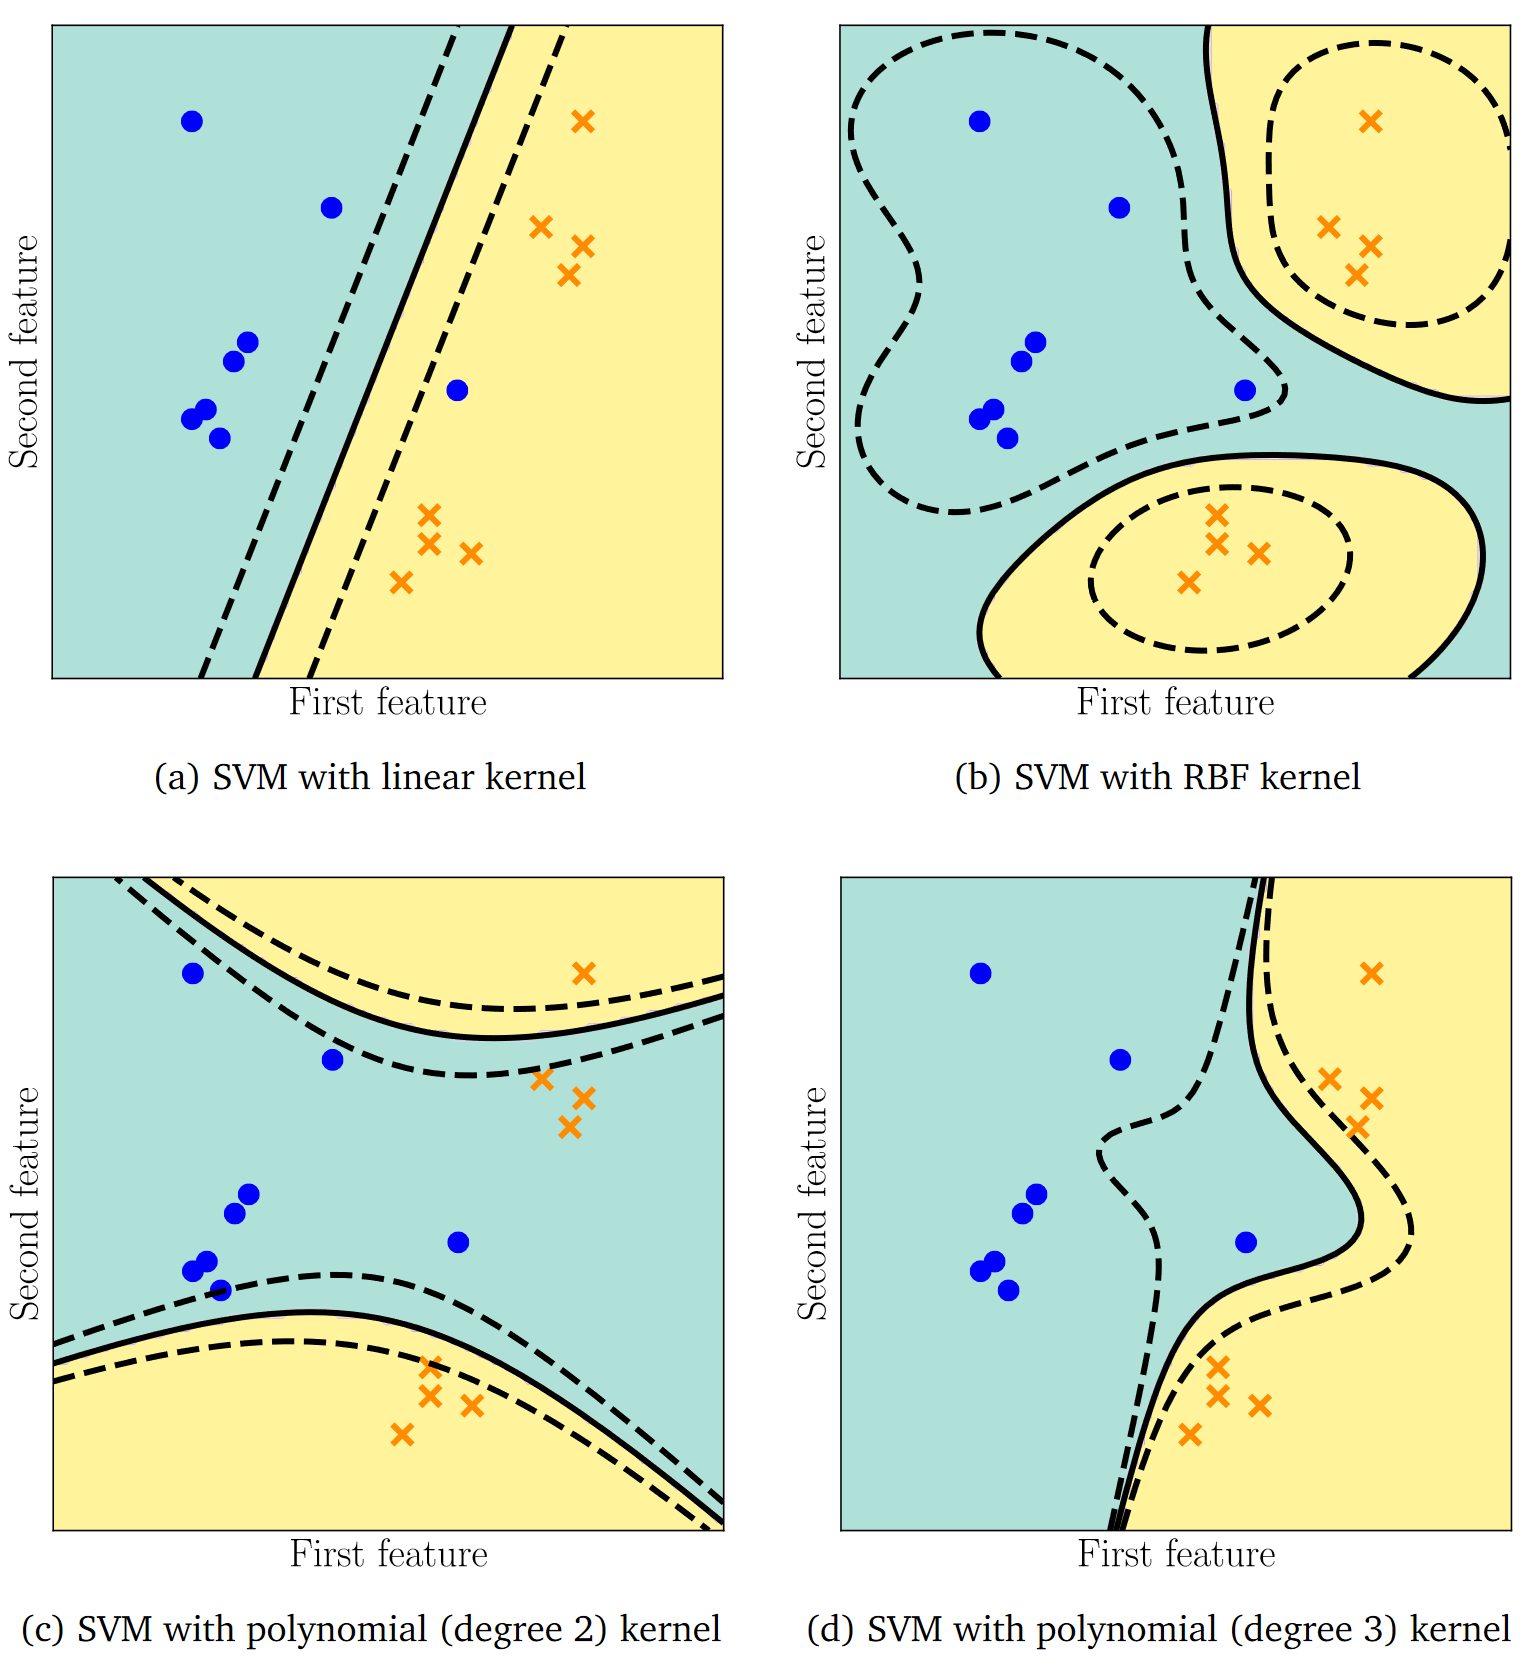
\includegraphics[width=0.7\linewidth]{img/ch4/kernels.png}
    \caption{Input space decision boundary of SVM with different kernels. Source (\cite{deisenroth_mathematics_2020}).}
    \label{fig:ch4.kernels}
\end{figure}


\subsection{The kernel trick}

Recalling the SVM formulation with regularization, equation \ref{eq:svm_primal_reg}, what we want to do now is to use a feature map such that the SVM operates on the feature space instead of the input space. If we modify every instance $\vb{x}$ with $\phi(\vb{x})$, replace the dot product with the inner product, and produce the dual using the Lagrangian method over this new formulation, we will obtain:
\begin{align*}
    \underset{\vt{\alpha}}{\text{arg} \max}\ \sum \alpha_i - \frac{1}{2} \sum \sum \alpha_i \alpha_j y_i y_j \ip{\phi(\vt{x_i}), \phi(\vt{x_j})}
    \text{\quad s.t. \quad} \forall \alpha_i : 0 \le \alpha_i \le C \land \sum \alpha_i y_i = 0
\end{align*}

Notice that with this new formulation we can replace the inner product with a kernel function and profit from all the advantages that kernels provide over having to explicitly compute the inner product in the feature space. This is called the “kernel trick”.

\subsubsection*{SVM Dual form (kernel version)}
\begin{align}\label{eq:svm_dual_kernel} 
    \underset{\vt{\alpha}}{\text{arg} \max}\ \sum \alpha_i - \frac{1}{2} \sum \sum \alpha_i \alpha_j y_i y_j k(\vb{x_i}, \vb{x_j})
    \text{\ \ \ s.t. \ \ } \forall \alpha_i : 0 \le \alpha_i \le C \land \sum \alpha_i y_i = 0
\end{align}

With this new version we also have the possibility to precompute all values of the kernel. We do this by defining a matrix $K_{i,j} = k(\vb{x_i}, \vb{x_j})$ called \emph{Gram matrix} or sometimes \emph{kernel matrix}. Because of the properties of kernels, a kernel matrix will always be symmetric and positive semi-definite, i.e. $\forall \vb{z} \in \mathbb{R}^n : \vb{z}^T K \vb{z} \ge 0$.

In the context of image processing, a convolution between a kernel matrix (also called \emph{convolution matrix}) and an image is used to do all kinds of filtering, including blurring, sharpening, embossing, edge detection, and more. This specific kernel matrix is generated using all discrete points representing pixel positions (the center of cells in a grid) with an origin in the center of the grid.

Another advantage of using kernels is that, since they don't restrict the input space to real numbers, you can now use SVM to classify between all kind of objects, e.g. sets, sequences, strings, graphs and distributions.

\section{SVM-RFE}

\begin{algorithm}[H]
    \DontPrintSemicolon
      %\KwInput{$p$}
      \KwOutput{$\vt{r}$}
      \KwData{$X_0,\vt{y}$}
      $\vt{s} = [1,2, \dotsc, n]$ \tcp*{subset of surviving features}
      $\vt{r} = []$ \tcp*{feature ranked list} 
      \While{$|\vt{s}| > 0$}
        {
            \tcc*[h]{Restrict training examples to good feature indices}\\
            $X=X_0(:,\vt{s})$\VS

            \tcc*[h]{Train the classifier}\\
            $\vt{\alpha} = \texttt{SVM-train(} X, y \texttt{)}$\VS

            \tcc*[h]{Compute the weight vector of dimension length $|\vt{s}|$}\\
            $\vt{w} = \sum_k{\vt{\alpha_k} \vt{y_k} \vt{x_k}}$\VS

            \tcc*[h]{Compute the ranking criteria}\\
            $\vt{c} = [(w_i)^2 \text{ for all $i$}]$\VS

            \tcc*[h]{Find the feature with the smallest ranking criterion}\\
            $f = \texttt{argmin($\vt{c}$)}$\VS

            \tcc*[h]{Update the feature ranking list}\\
            $\vt{r} = [\vt{s}(f), ...\vt{r}]$\VS

            \tcc*[h]{Eliminate the feature with smallest ranking criterion}\\
            $\vt{s} = [...\vt{s}(1:f - 1), ...\vt{s}(f + 1:|\vt{s}|)]$
        }
    \caption{SVM-RFE}
\end{algorithm}

----

\begin{itemize}
    \item What is RFE.
    \item The ranking criteria for the linal case.
\end{itemize}

\begin{algorithm}[H]
    \DontPrintSemicolon
      \KwInput{$t$ \tcp*{t = step}}
      \KwOutput{$\vt{r}$}
      \KwData{$X_0,\vt{y}$}
      $\vt{s} = [1,2, \dotsc, n]$ \tcp*{subset of surviving features}
      $\vt{r} = []$ \tcp*{feature ranked list} 
      \While{$|\vt{s}| > 0$}
        {
            \tcc*[h]{Restrict training examples to good feature indices}\\
            $X=X_0(:,\vt{s})$\VS

            \tcc*[h]{Train the classifier}\\
            $\vt{\alpha} = \texttt{SVM-train(} X, y \texttt{)}$\VS

            \tcc*[h]{Compute the weight vector of dimension length $|\vt{s}|$}\\
            $\vt{w} = \sum_k{\vt{\alpha_k} \vt{y_k} \vt{x_k}}$\VS

            \tcc*[h]{Compute the ranking criteria}\\
            $\vt{c} = [(w_i)^2 \text{ for all $i$}]$\VS

            \tcc*[h]{Find the $t$ features with the smallest ranking criterion}\\
            $\vt{f} = \texttt{argsort}(\vt{c})(\ :t)$\VS

            \tcc*[h]{Update the feature ranking list}\\
            $\vt{r} = [\vt{s}(\vt{f}), ...\vt{r}]$\VS

            \tcc*[h]{Eliminate the features with the $t$ smallest ranking criterion}\\
            $\vt{s} = [[...\vt{s}(1:f_i - 1), ...\vt{s}(f_i + 1:|\vt{s}|)]$ for all $i]$
        }
    \caption{SVM-RFE with Step}
\end{algorithm}
